\section{Introduzione}

%-----------------------------------------%
%				Prima slide				  %
%	Hamiltoniana di Ising e spiegazione	  %
%-----------------------------------------%
\begin{frame}
    \frametitle{Hamiltoniana}
    \framesubtitle{}

    \begin{columns}
        \begin{column}{0.5\textwidth}
			
			\vspace{12pt}

			\begin{equation*}
				H\,=\,-J\sum_{\left<i,j\right>}\sigma_i\sigma_j\,-\,h\sum_{i} \sigma_i
				\label{eq: Ham_Ising}
			\end{equation*}

			\vspace{12pt}

            \begin{itemize}[itemsep=0.5em, label=$\diamond$]
                \item Interazione fra primi vicini
                \item Accoppiamento con un campo esterno
            \end{itemize}

        \end{column}

        
        \begin{column}{0.5\textwidth}
				\centering
				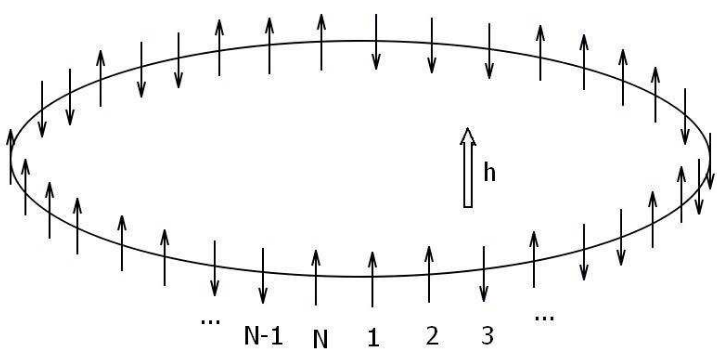
\includegraphics[width=\textwidth]{Immagini/Introduzione/modelloIsing1D_pbc.png}
				{\scriptsize Modello di Ising 1D con condizioni periodiche.}
		
		\end{column}
      \end{columns}
  
\end{frame}



%----------------------------------------------%
%			  Seconda slide				       %
%	Modello di Ising 1D e soluzione analitica  %
%----------------------------------------------%
\begin{frame}
    \frametitle{Modello di Ising 1D}
    \framesubtitle{}

    \begin{columns}

        \begin{column}{0.5\textwidth}
			
			\vspace{12pt}

			\begin{itemize}[itemsep=0.5em, label=$\diamond$]
                \item Teoria di campo medio
                \item Sistema presenta una transizione di fase a $T_c \neq 0$
            \end{itemize}

			\vspace{12pt}

			\begin{equation*}
				m\,=\,\tanh{\left[\beta\left(h\,+\,Jn_{nn}m\right)\right]}
				\label{eq: magn_Ising1D_MF}
			\end{equation*}

        \end{column}


        \begin{column}{0.5\textwidth}
			
			\vspace{12pt}

			\begin{itemize}[itemsep=0.5em, label=$\diamond$]
                \item Soluzione analitica
                \item Sistema disordinato per ogni $T\,\neq\,0$ a campo esterno nullo
            \end{itemize}

			\vspace{12pt}

			\begin{equation*}
				m\,=\,\frac{\sinh{\left(\beta h\right)}}{\sqrt{e^{-4\beta J}\,+\,\sinh^2{\left(\beta h\right)}}}
				\label{eq: magn_Ising1D_AS}
			\end{equation*}

        \end{column}
      \end{columns}
  
\end{frame}



%----------------------------------------------%
%			     Terza slide			       %
%	Modello di Ising 2D e transizione di fase  %
%----------------------------------------------%
\begin{frame}
    \frametitle{Modello di Ising 2D}
    \framesubtitle{}

    \begin{columns}

        \begin{column}{0.55\textwidth}

			\begin{itemize}[itemsep=0.5em, label=$\diamond$]
                \item Soluzione analitica per $h = 0$
                \item Sistema presenta una transizione di fase a $T_c \neq 0$
            \end{itemize}

			\begin{equation*}
				m\left(\beta,\,h=0\right)\,=\,
				\begin{cases}
				\left[1\,-\,\dfrac{1}{\sinh^4{\left(2\beta J\right)}}\right]^{\frac{1}{8}}\,\, T\,<\,T_c \\
				0 \qquad \qquad \qquad \qquad \,\,\,\, T\,>\,T_c
				\end{cases}
				\label{eq: magn_Ising2D_AS}
			\end{equation*}

        \end{column}
        
        \vspace{0.3cm}

        \begin{column}{0.45\textwidth}
			
			\centering
            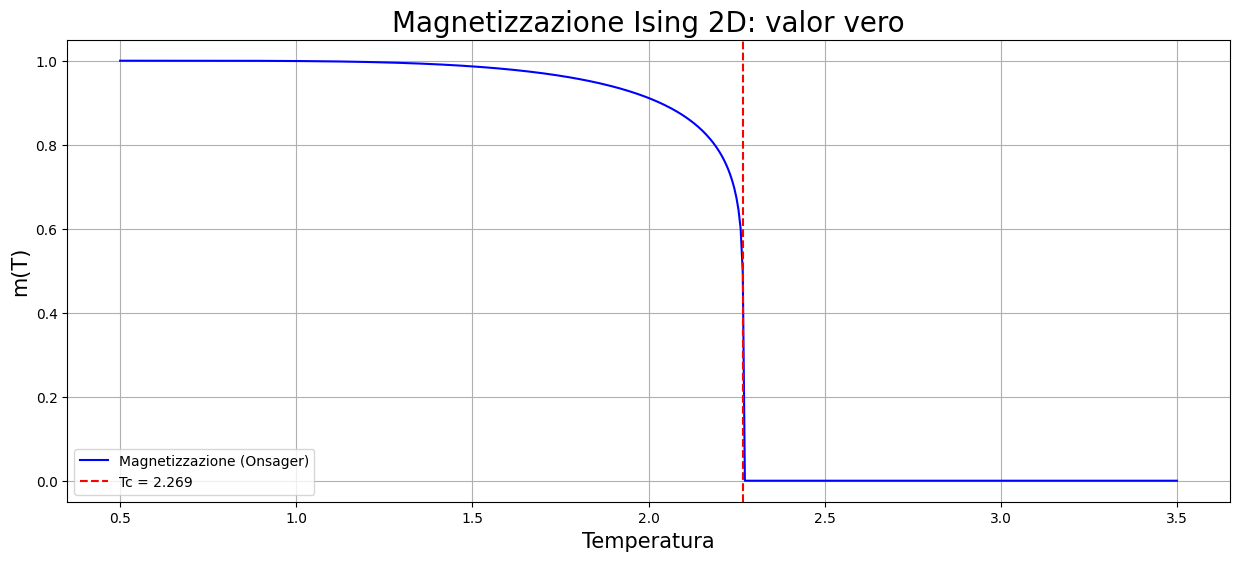
\includegraphics[width=\textwidth]{Immagini/Introduzione/magn_Ising2D.png}

            \begin{tabular}{cc}
                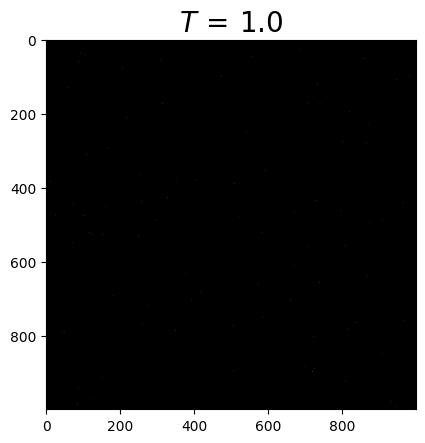
\includegraphics[width=0.45\textwidth]{Immagini/Introduzione/cg_1000_1.0.png} &
                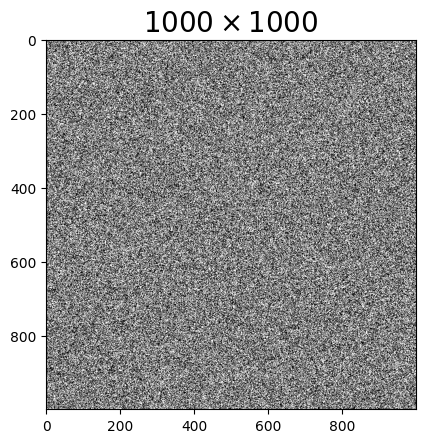
\includegraphics[width=0.45\textwidth]{Immagini/Introduzione/cg_1000_3.0.png} \\
            \end{tabular}
        
        \end{column}
      \end{columns}
  
\end{frame}
